\chapter{Implementation}

\section{Directory Structure}
The directory structure (for the application only) is defined as follows:

\begin{itemize}
    \item \textbf{app} contains various Laravel application components, such as models, controllers, and policies
    \item \textbf{bootstrap} Framework code used by Laravel to bootstrap the application
    \item \textbf{config} Framework code that define configurations for various Laravel utilities and functionalities
    \item \textbf{database} Database factories, migration definitions, and seeding tools are in this directory.
    \item \textbf{docs} Documentation generated by Sami is stored here. This is explored in more detail in Chapter 7.
    \item \textbf{node\_modules} This contains Node.js dependencies installed by Laravel Mix and are used in development. This is discussed in greater detail in Chapter 7.
    \item \textbf{public} is the front-facing directory containing the application entry-point, as well as compiled assets and images used for social media.
    \item \textbf{routes} HTTP Application routes are defined in the files contain within this directory.
    \item \textbf{resources} Views written in Laravel Blade are kept in this folder, along with stylesheets and scripts that comprise the front-end.
    \item \textbf{storage} Laravel stores log files here, and generated PDF files for download are kept here. A cache for quick loading is also stored here.
    \item \textbf{tests} PHPUnit tests are kept here, and are covered in Chapter 6.
    \item \textbf{vendor} Similar to \textit{node\_modules}, this folder stores PHP dependencies used by Laravel, as well as additional third-party libraries.
\end{itemize} \cite{W3Schools1}

\section{Method of Action}
The Laravel developers acknowledge that having a basic, high-level understanding of how a framework works is important for not only having a basic grasp of how the application works, but also to make 'everything feel less magical'. \cite{Laravel6} This is important as frameworks are characterised by carrying out substantial amounts of work for you, in order to drastically reduce development time and to produce better quality applications, and are generally recommended by the greater web development community. \cite{Mozilla3}

\begin{figure}[!ht]
    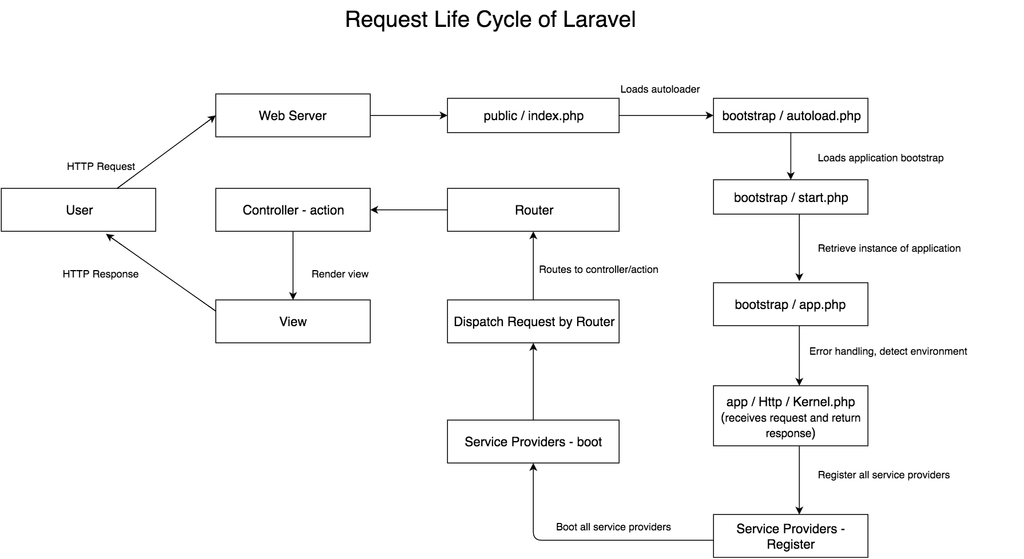
\includegraphics[width=1.0\textwidth]{Figures/laravel-request}
    \caption{Diagram that shows how the Request Lifecycle for the Laravel framework operates.}
    \label{fig:laravel-requests} \cite{Mallow1}
\end{figure}

When a HTTP (Hypertext Transfer Protocol) request is received by the web server by navigating to the \textbf{index.php} file in the \textit{public} directory, the application is quickly bootstrapped, loading all necessary libraries and components by means of the PSR-4 autoload file, which is a widely accepted PHP coding standard and was generated by Composer, the PHP package manager when the application was first installed. \cite{PSR1} From here, the application can determine how to 'route' the request based on route definitions and the URL (Uniform Resource Locator) path, delegating actions to the appropriate controllers and their models defined in those definitions, before passing data to a view, and returning it to the user. \cite{Laravel6} According to Stauffer, Laravel's approach 'brings your ideas to reality with no wasted code' and 'modern programming standards.' \cite{LaravelUp1}

\section{HTTP Routes}

\begin{figure}[!ht]
    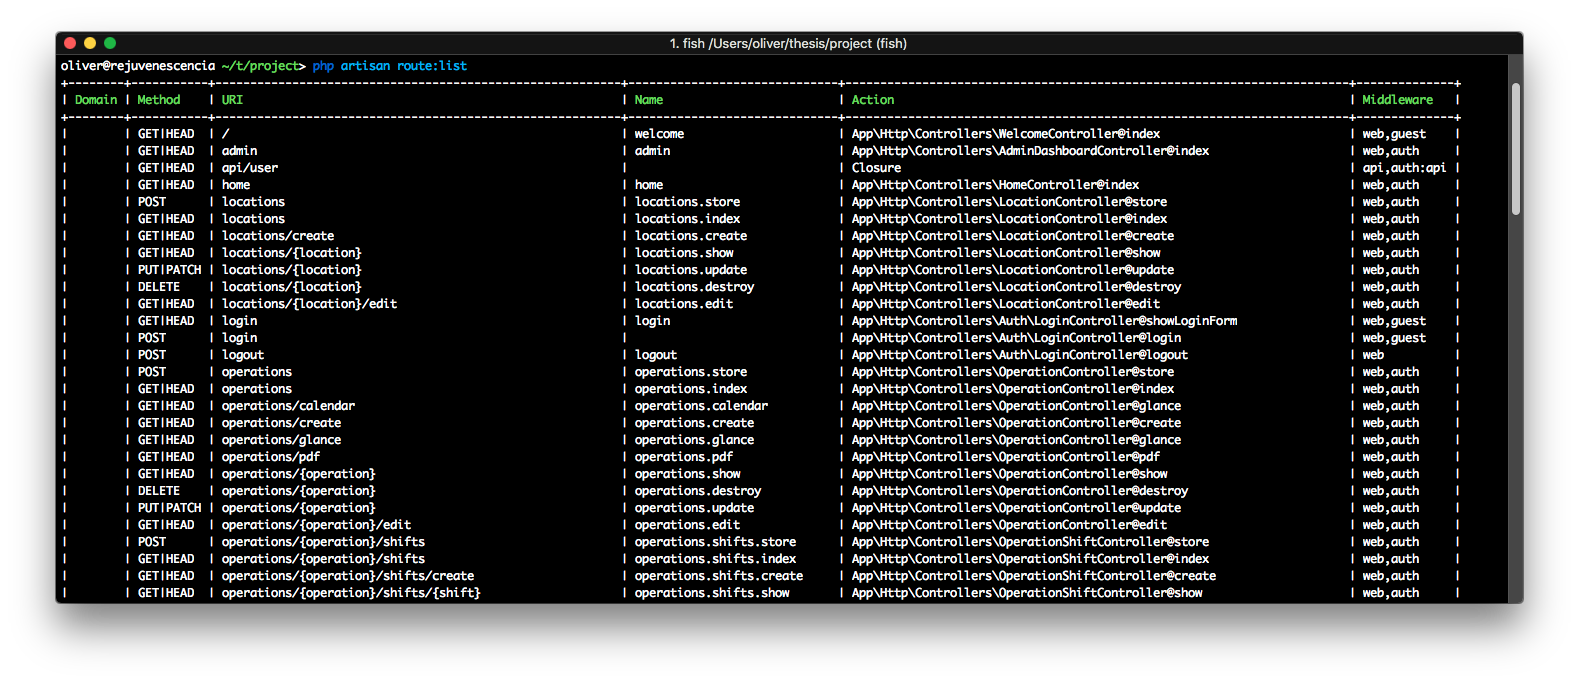
\includegraphics[width=1.0\textwidth]{Figures/routes}
    \caption{A print out of HTTP routes defined within the application, their corresponding URLs, associated controllers and methods, and HTTP actions.}
    \label{fig:methods}
\end{figure}

The controllers for each resource (i.e. users, operations) as well as individual webpages uses a RESTful (Representational State Transfer) architecture, and have methods that correspond to the CRUD verbs - create, read, update, and delete. There are also additional methods that help facilitate the CRUD operations, such as 'show' for viewing individual entries, and 'edit' to display a form in order to modify an existing record. Different actions may expect different HTTP requests, such as GET, POST, PATCH, and DELETE respectively. Each action, whether viewing one's own profile, editing a user's profile, registering for a shift, or deleting an operation, are all represented by their own route within the application, including custom defined routes that do not correspond to CRUD, such as those used for (de)registering to an operation. \cite{Laravel7} \cite{7539825}

\section{Models and Relationships}

\begin{figure}[!ht]
    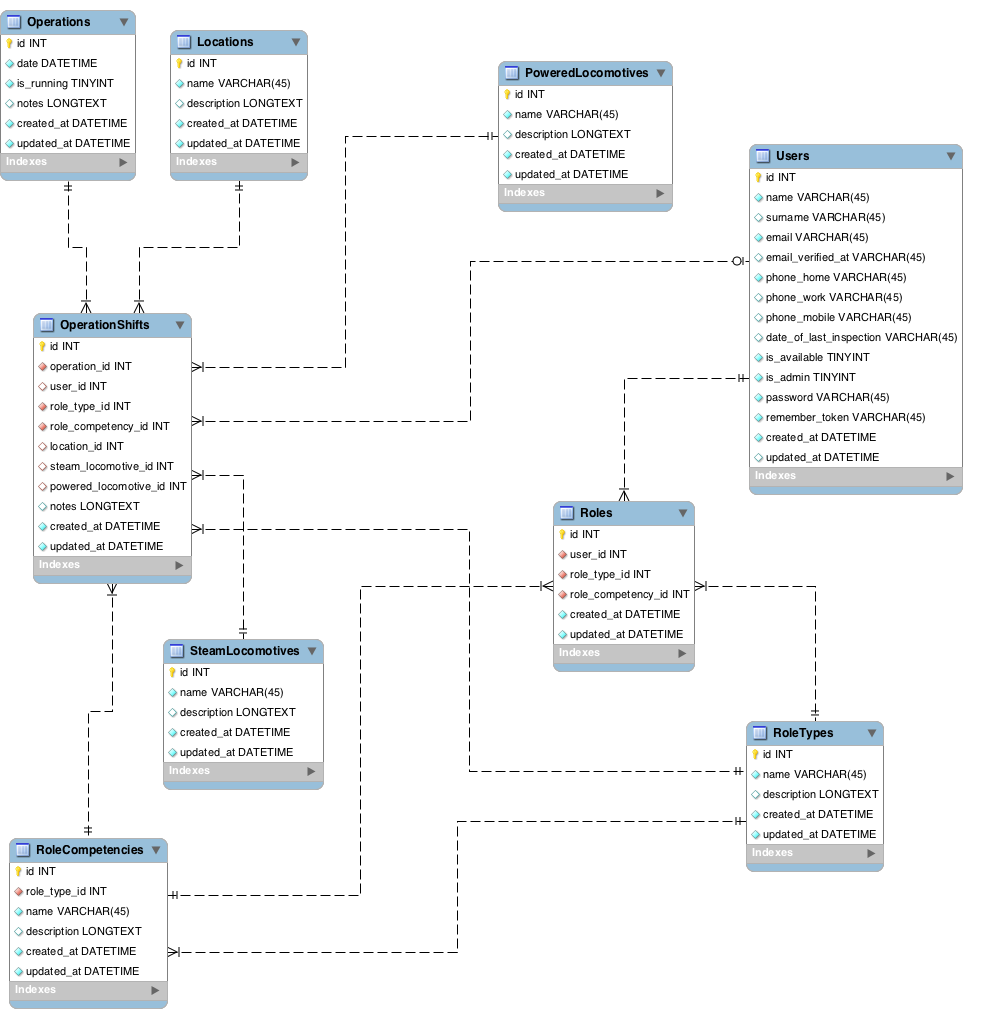
\includegraphics[width=1.0\textwidth]{Figures/Models}
    \caption{UML diagram showing the relationships between database tables and their structure. The relationships are defined by their Eloquent relationships.}
    \label{fig:relationships}
\end{figure}

Database models define their column names and data types within migration files, alongside foreign keys, their references, and any constraints. As shown by Figure \ref{fig:relationships}, many of the tables belong to shifts, as each shift can have corresponding vehicles associated with it, a designated location, a required role and competency level, as well as the volunteer that is assigned to that volunteer, which is of course null when the shift is vacant.

\section{Views and Laravel Blade}

Controller methods, as part of their response to the user's request will return a view that can be populated with data processed or retrieved, such as returning the current resource object for display when viewing an individual item, like a role type. Laravel uses a language called Blade for its templating engine, which allows for reusable front-end code, and more legible syntax for inserting data into views or extending existing template files than using raw PHP alone, though vanilla PHP script is nevertheless supported and will be interpreted all the same. \cite{Laravel9} \cite{Underwood1}

An example of a data being passed to a view can be seen in the following code, that is taken from the controller for operations, where all operations retrieved from the database (by Eloquent) are injected into the view as an argument, to be parsed and displayed there:

\begin{lstlisting}[language=PHP, breaklines]
    public function index()
    {
        $operations = Operation::orderBy('date', 'desc')->paginate(3);
        return view('operation.index', compact('operations'));
    }
\end{lstlisting}

The name of the view to be rendered by Laravel is 'operation.index', which will now have access to the contents of \texttt{\$operations}. In the following snippet of Blade code, you can see the contents of this variable being iterated through and printed in tabular form, as well as the usage of vanilla PHP script where it has been deemed necessary:

\begin{lstlisting}[language=HTML, breaklines]
    <tbody>
    @foreach ($operations as $operation)
        @php
            $operationDate = \Carbon\Carbon::parse($operation->date);
        @endphp
        <tr>
        ...
        </tr>
        ...
    @endforeach
    </tbody>
\end{lstlisting}

\section{Users}

\begin{figure}[!ht]
    \centering
    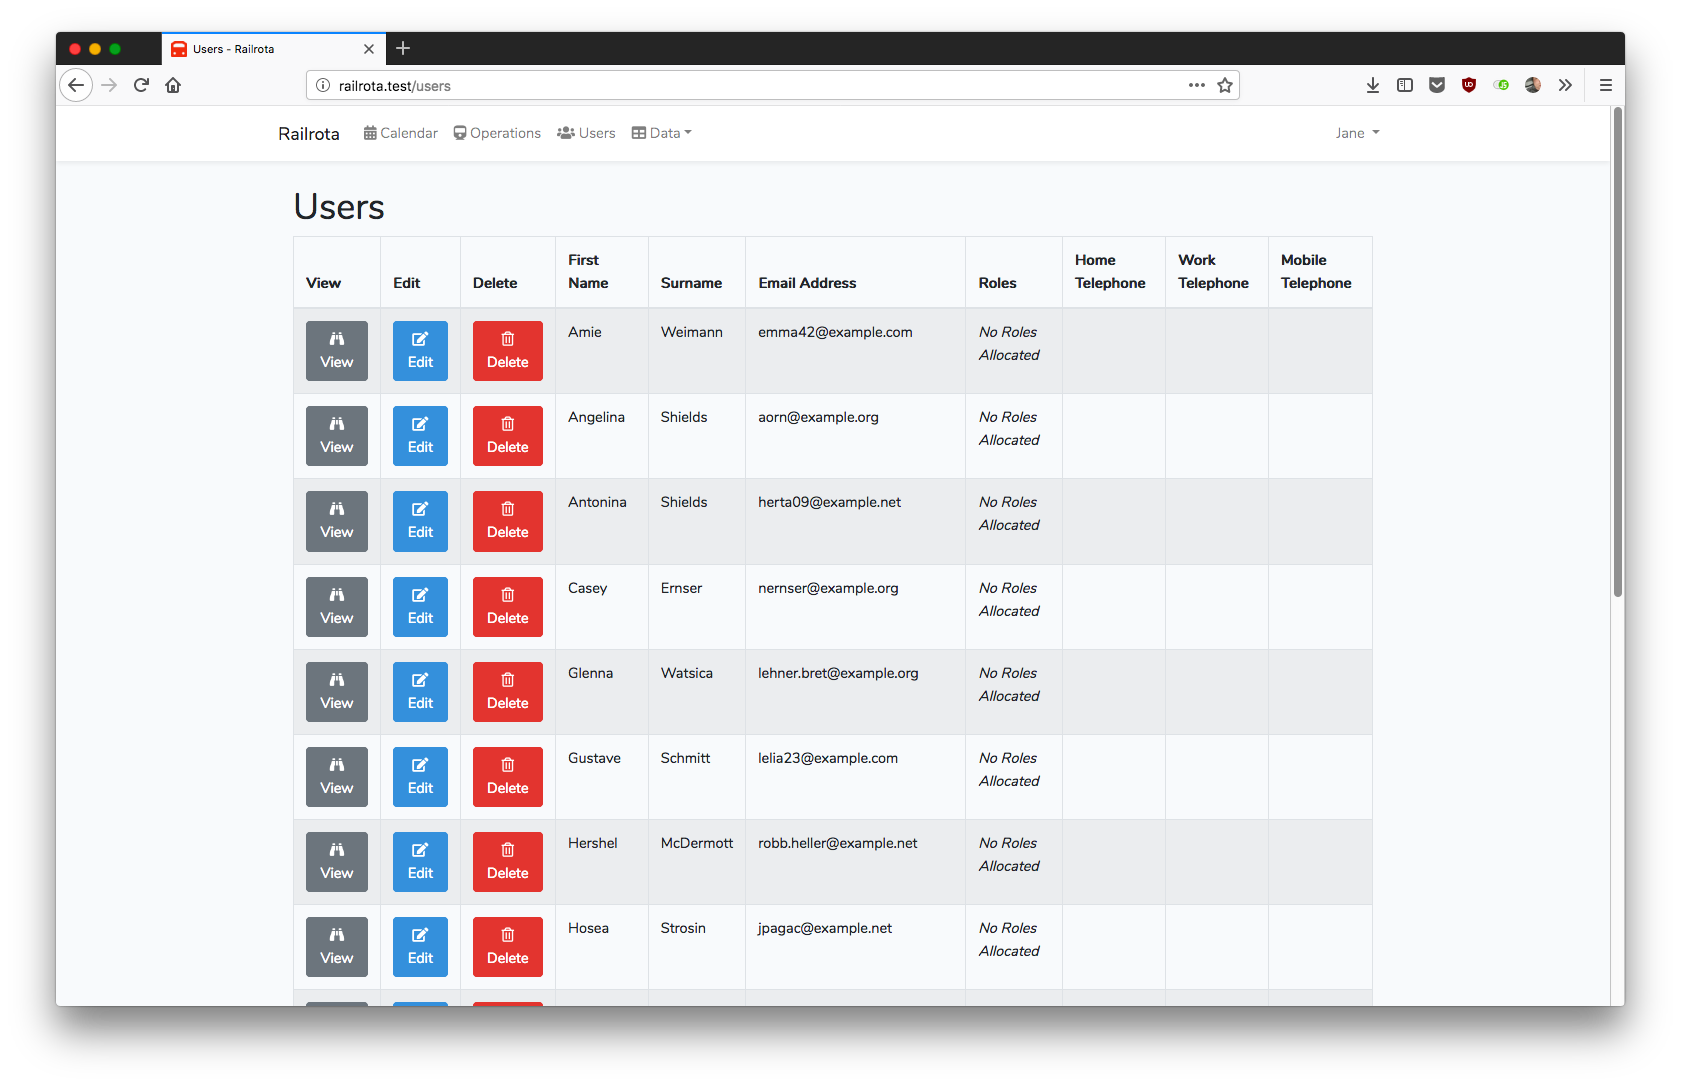
\includegraphics[width=1.0\textwidth]{Figures/screenshot-users}
    \caption{Screenshot of the Users interface within the application.}
    \label{fig:users}
\end{figure}

All volunteers are users within the application, with users that have access to administrative privileges being denoted by a boolean true value in \textbf{is\_admin}. Users can modify a subset of their own information, but are unable to assign themselves roles or privileges, or modify a date value indicating the last time they were inspected.

\begin{figure}[!ht]
    \centering
    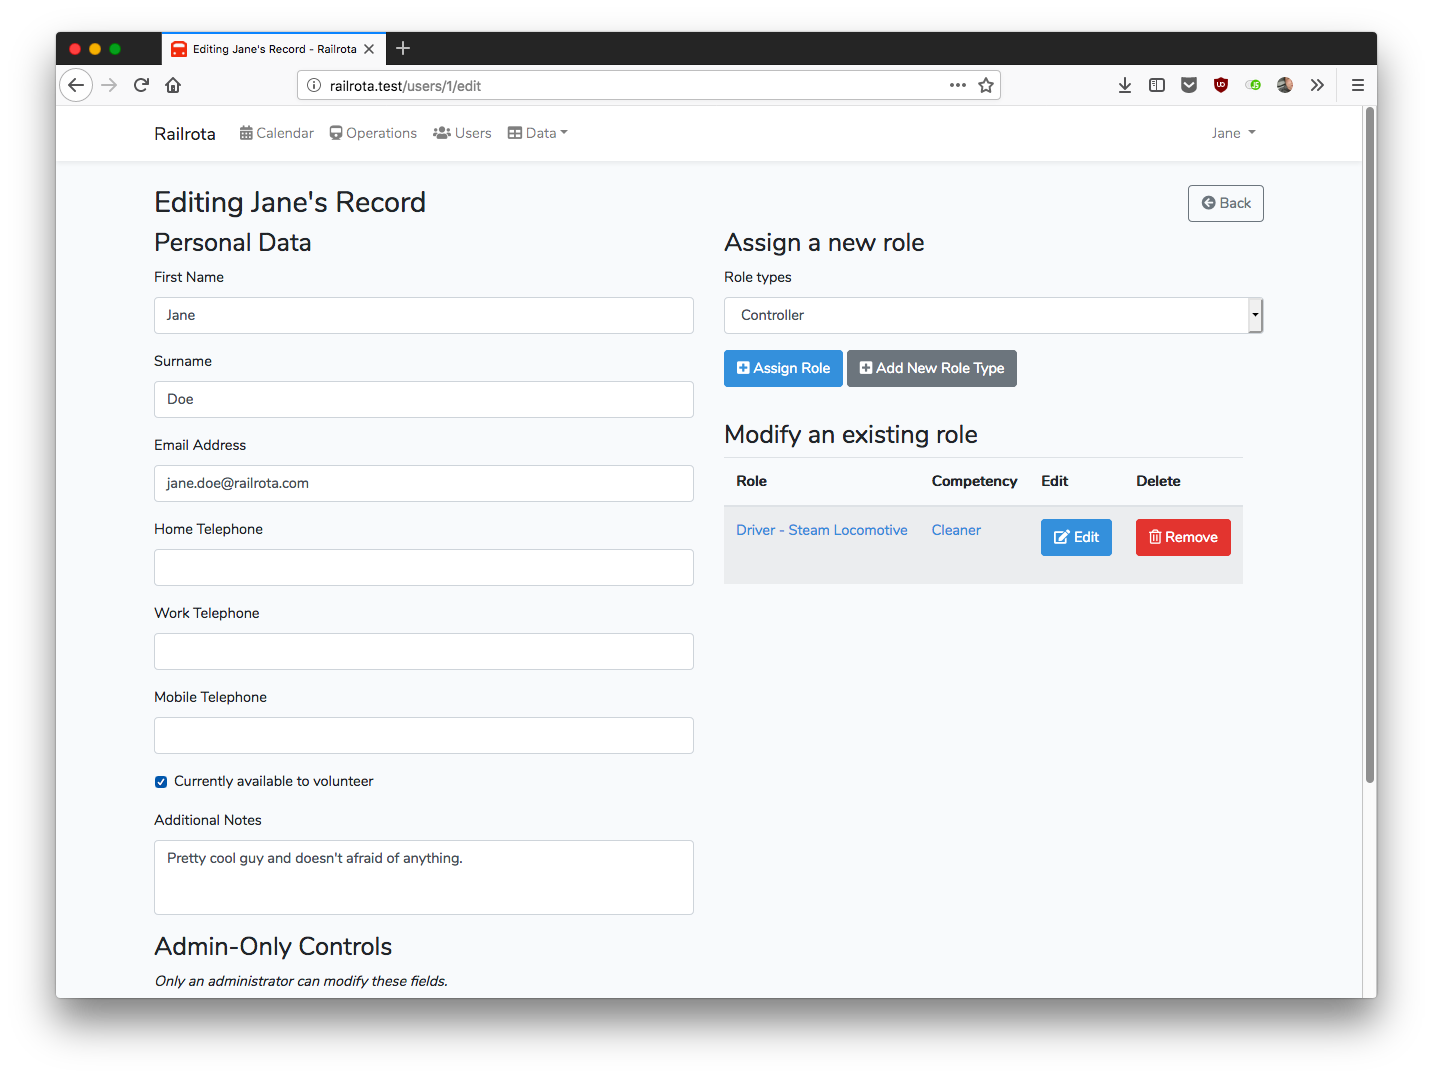
\includegraphics[width=1.0\textwidth]{Figures/screenshot-edit-user}
    \caption{Screenshot of the Edit User interface, as seen by an administrator.}
    \label{fig:users-edit}
\end{figure}

The following destroy CRUD method in the User controller, demonstrates how after checking the policies that the current user is authorised to delete a user (so is an administrator), it checks first whether they are attempting to delete themselves, which is understandably undesirable behaviour, and redirects back with an error message if this is the case. Otherwise, the \textbf{delete} Eloquent method is called on the user object, and it is deleted from the database; redirecting back with a success notification. The User object is resolved from the unique ID in the URL. \cite{Laravel7}

\begin{lstlisting}[language=PHP, breaklines]
    public function destroy(User $user)
    {
        $this->authorize('delete', $user);

        if ($user->id === Auth::id()) {
            flash()->error('You can\'t delete yourself!')->important();
            return redirect()->back();
        }

        $user->delete();
        flash()->success("{$user->name} has been deleted successfully!")->important();
        return redirect()->route('users.index');
    }
\end{lstlisting}

\subsection{Authentication}
Authentication functionality can be scaffolded seamlessly by Laravel by issuing the \texttt{php artisan make:auth} command at on the command line, and provides all the necessary registration, login, and password reset functionality - and automatically ties this into the User model.

By declaring routes within the authentication middleware group as the following code demonstrates, Laravel will ensure that a user is authenticated in order to access any of the routes contained therein, otherwise redirecting back to the login page. \cite{Laravel8}

\begin{lstlisting}[language=PHP, breaklines]
    Route::group(['middleware' => ['auth']], function() {
        Route::resource('users', 'UserController');
    }
\end{lstlisting}

\subsection{Authorisation and Policies}
Authorisation - determing who can and who cannot access resources or carry out certain actions is determined by classes known as policies within Laravel - where authorisation logic is stored. \cite{Larashout1} In this application, a policy is necessary wherever there are actions that users and administrators have different levels of access to, such as being able to create roles, operations, or modify user data.

A corresponding method is typically called in a controller's respective policy (i.e. UserController will have a matching policy called UserPolicy) and within the controller action itself, the appropriate method for that action is passed as an argument, alongside the currently authenticated user object, like thus:

\begin{lstlisting}[language=PHP, breaklines]
    $this->authorize('create', $user);
\end{lstlisting}

This calls the corresponding create method in its policy file, which will return either true for successful authorisation and allowing the remainder of the controller method to execute. Otherwise, the action is prevented. A call to this method absolutely must exist for any authorisation to occur, regardless of whether there is a corresponding policy class to the aforementioned controller and model. The corresponding 'create' policy method in the UserPolicy file is as follows:

\begin{lstlisting}[language=PHP, breaklines]
    public function create(User $user)
    {
        return $user->isAdmin();
    }
\end{lstlisting}

This simple but effective method calls a custom method on the model itself that returns whether or not the attribute \textbf{is\_admin} on the currently authenticated user is true or not. If the value isn't truthful, then execution halts as authorisation has subsequently failed.

\section{Role Types}

\begin{figure}[!ht]
    \centering
    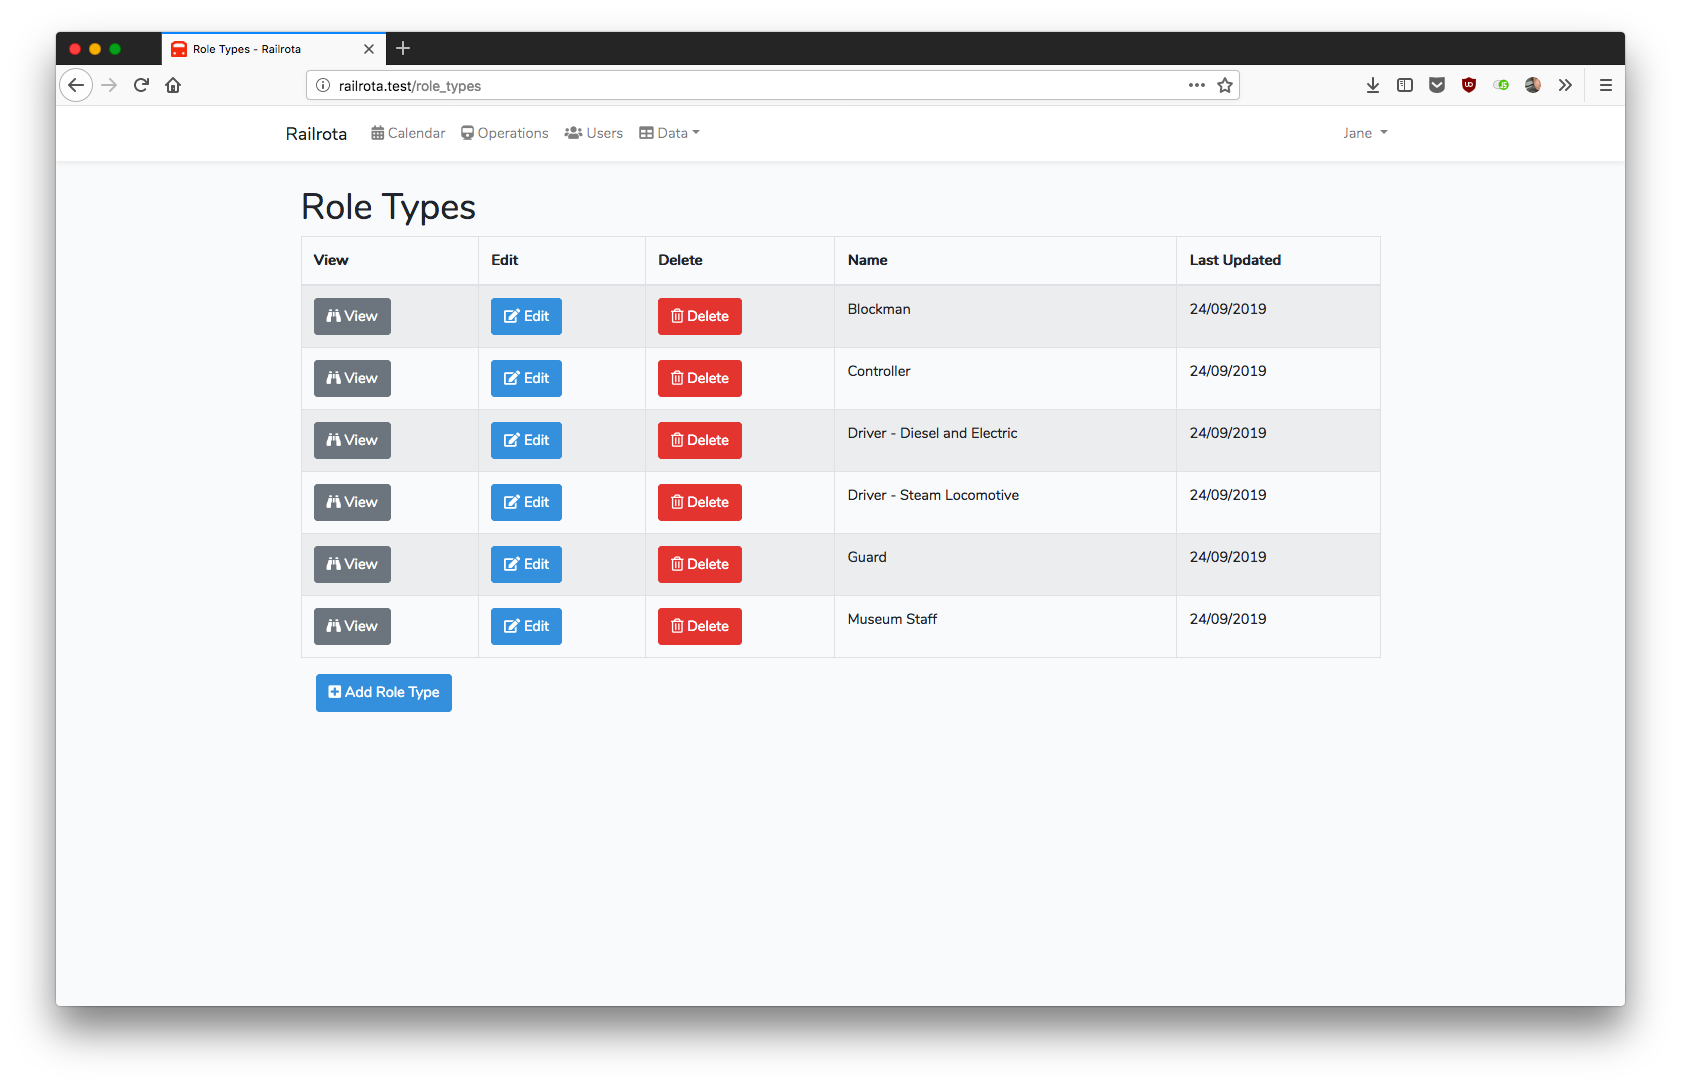
\includegraphics[width=1.0\textwidth]{Figures/screenshot-roletypes}
    \caption{Screenshot of the Role Types interface within the application.}
    \label{fig:roletypes}
\end{figure}

In order to volunteer for a shift, a user must have the relevant role type that is also shared by the shift. For example, a shift might have a \textit{Blockman} vacancy available, but in order to volunteer for the role, they need to have that role themselves. Role types are treated as resources with CRUD routes, and can only be modified in any form by administrators.

Role types are not hardcoded into the system, and are their own database table, although a list of defaults is defined in the source code that can be used during initial setup, and consist of the following roles: 

\begin{itemize}
    \item Controller
    \item Guard
    \item Blockman
    \item Driver (Diesel/Electric)
    \item Driver (Steam)
    \item Museum Staff
\end{itemize}

Additional role types can be added to the system to accommodate any future needs of the railway, or existing ones may be modified or deleted as necessary.

\section{Role Competencies}

\begin{figure}[!ht]
    \centering
    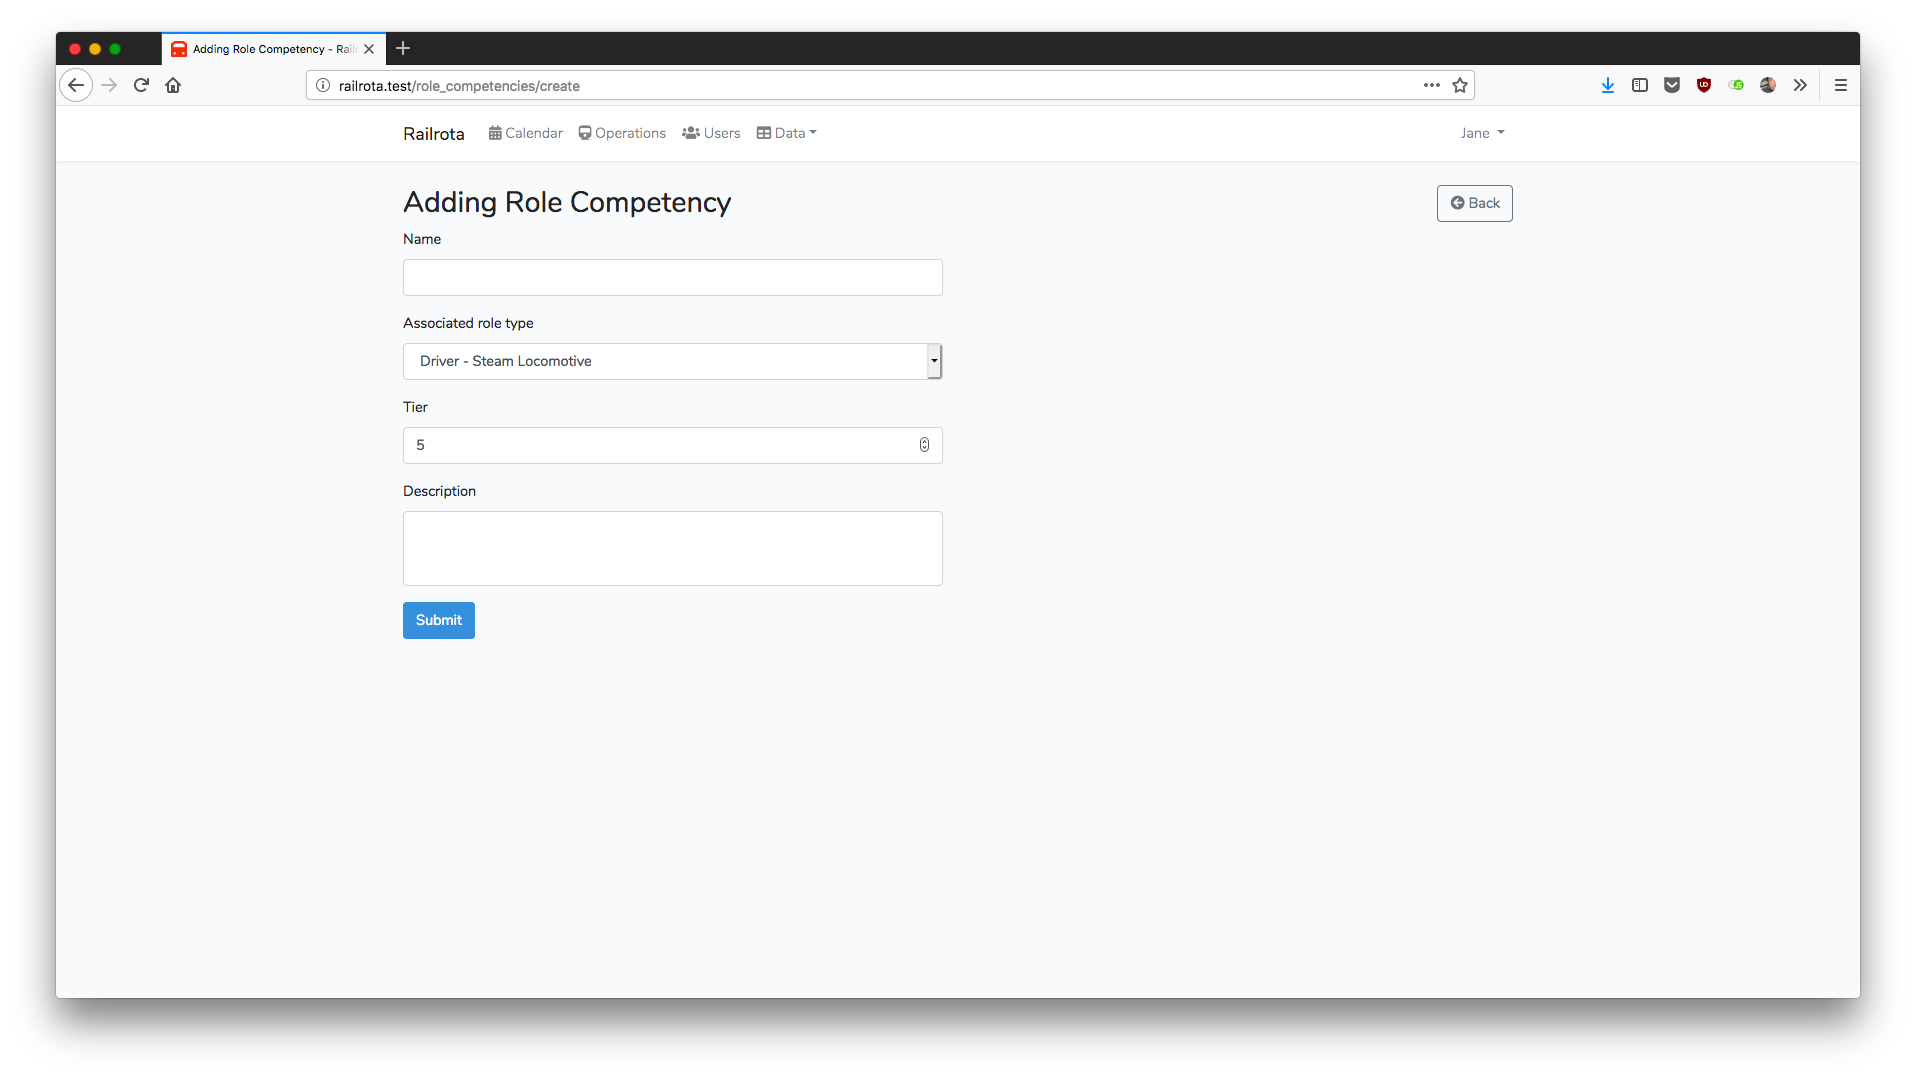
\includegraphics[width=1.0\textwidth]{Figures/screenshot-competency-create}
    \caption{Screenshot of an administrator adding a new competency level to the a driver role.}
    \label{fig:competencies-create}
\end{figure}

Each role can have multiple competency levels, each with their own tier between 1 and 10. Those with a competency in a specific role can volunteer for shifts equal or lesser to their numerical tier. 

For example, if there is a Blockman Shift requiring at least a Trainee, which have a numerical tier of 1, then those with Passed (2) or Examiner (3) can also sign up for the same work. If the shift required someone with Passed (2) level, then a Trainee (1) would not be able to register for it.

Each of the default role types have predefined default competencies also, but additional competencies can be added and those existing may also be modified. Furthermore, the numerical tiers are not unique, so multiple competencies for a role may share the same tier. Shifts can also not have tier requirements set, and can therefore be met by any level, including if a user does not have a competency level defined for whatever reason.

This algorithm that ensures that competency levels are met is explored in more detail in the Operations and Shift subsection.

\section{Roles}

A role type and role competency is linked to a user by means of a role - which can be viewed as properties of a user, as users can have multiple roles each with their own role type and role competency.

As they are used akin to a pivot table, tying information on the aforementioned tables together, there are no forms to directly create them, and the necessary controls to do so are only visible to an administrator on the respective user's edit UI, as shown by figure \ref{fig:users-edit}.

\section{Locations and Locomotives}

\begin{figure}[!ht]
    \centering
    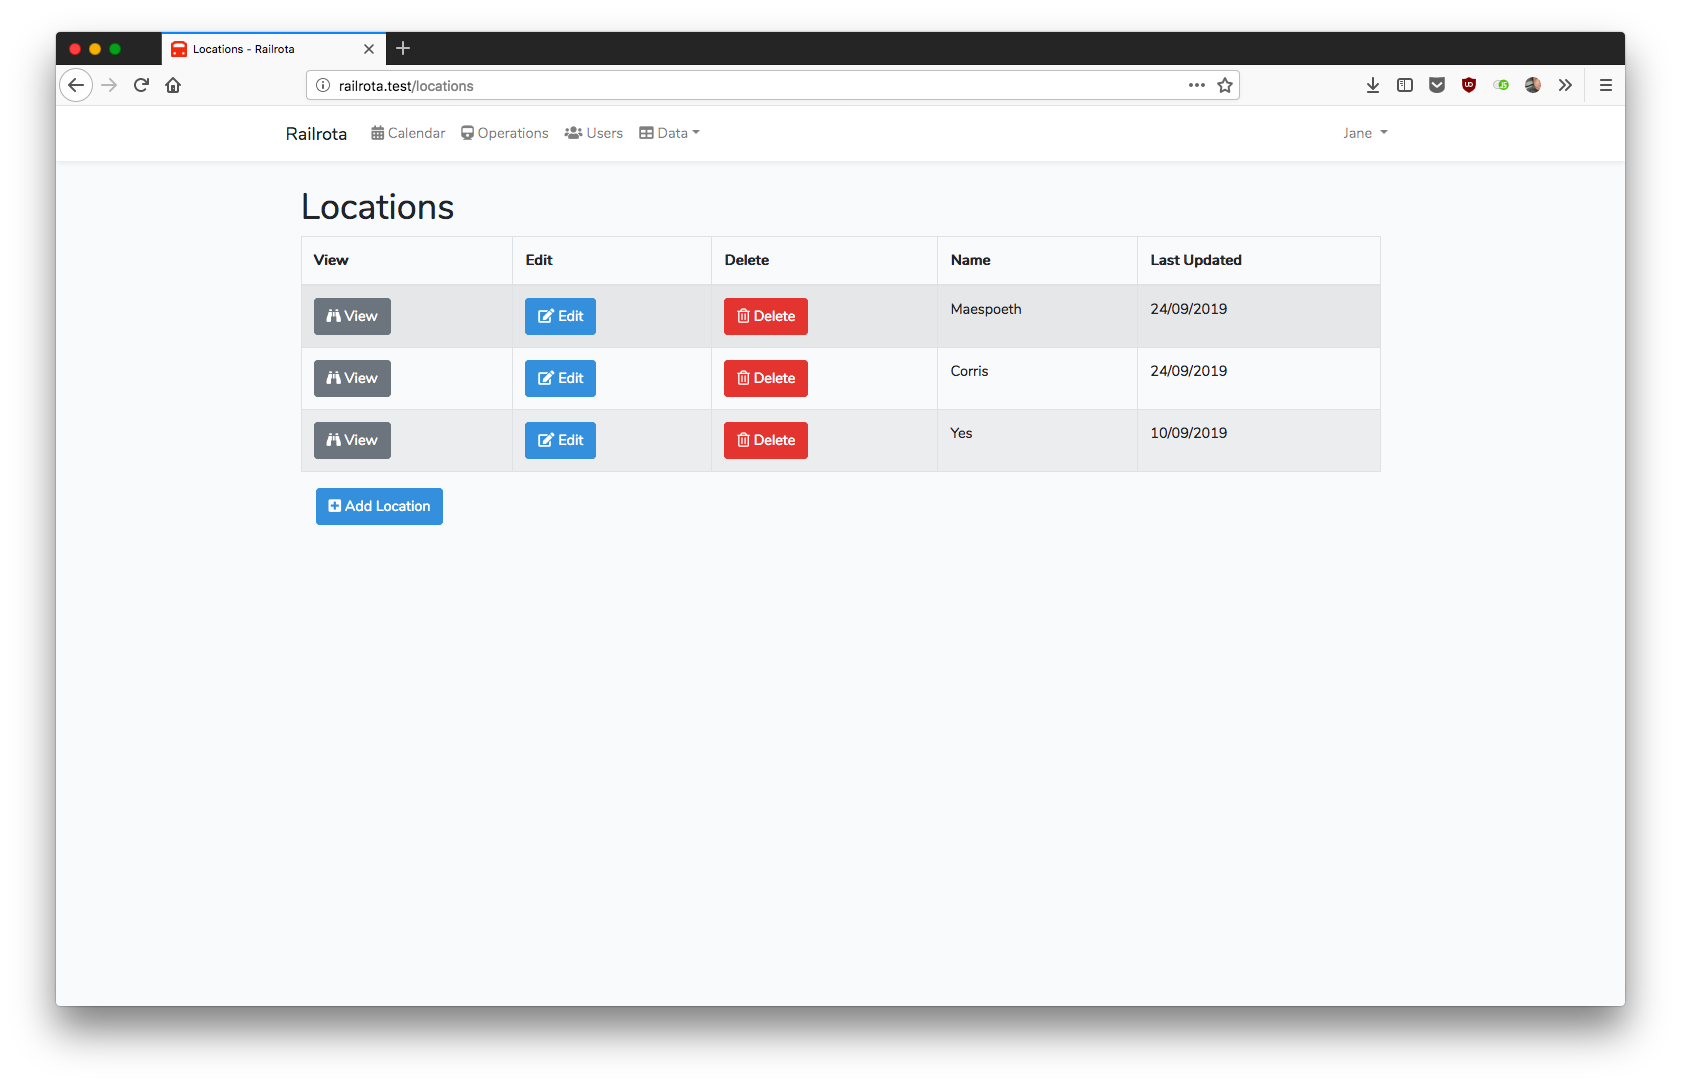
\includegraphics[width=1.0\textwidth]{Figures/screenshot-locations}
    \caption{Screenshot of locations being listed within the application, which is viewable by all users.}
    \label{fig:locations}
\end{figure}

Locations and two types of Locomotives, both Steam and Diesel/Electric are all individual tables in the database but have been grouped for the sake of brevity, as they all function in an identical way, with the only difference being that they have different default values that can be used during initial set up. The information is minimal - the name, an optional description, and timestamps.

Shifts can have optional location information, providing information to users where a shift is located (i.e. what station or railway, or some other geographical location) and if it involves a vehicle, such as a steam locomotive, which one. These resources can only be created or manipulated by administrators, but users can view information about them in the same way they may view other resource data.

When deleting any of these nullable resources, shifts that point to affected table entries will also be nulled.

\section{Operations and Shifts}

\begin{figure}[!ht]
    \centering
    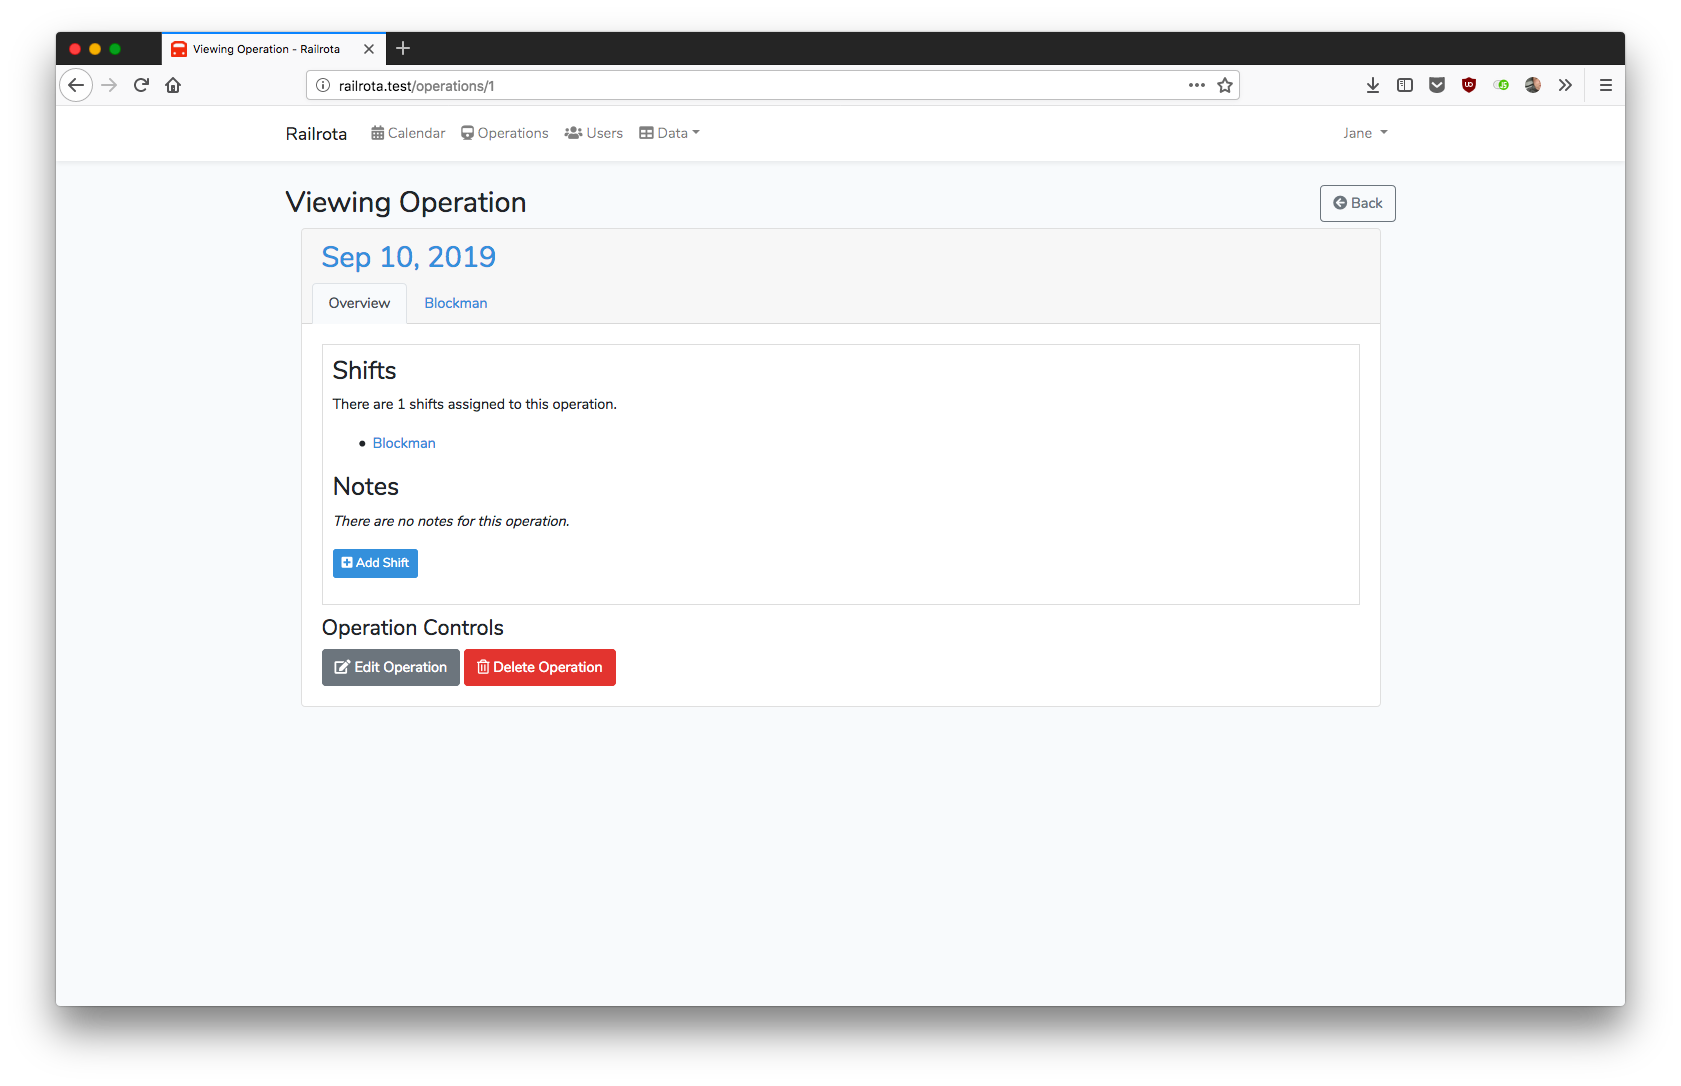
\includegraphics[width=1.0\textwidth]{Figures/screenshot-operations}
    \caption{Screenshot of the operations interface, containing one shift and administrative controls.}
    \label{fig:operations}
\end{figure}

Operations are each individual day where the railway will be operating, and each operation can have an unlimited amount of shifts. A shift is a specific volunteering vacancy, with its only requirement being the role type, i.e. what kind of work is required for that shift. Additional information such as location, locomotives, and competencies can also be specified, but are optional. Users can be manually assigned to shifts on creation, such as if an administrator knows in advance that a volunteer is to staff a certain shift, which can, with warning, override any typically enforced role requirements.

In a nutshell, an operation can be thought of as a workday, with each vacancy therein being an individual shift. This system is inspired by the exisitng system showed in Appendix \ref{Example Timetable} and additional domain knowledge examined from research into the HOPS platform. \cite{Hops2} If the operation is declared closed for whatever reason, such as understaffing of critical volunteers, it is impossible for users to sign up for shifts.

\begin{figure}[!ht]
    \centering
    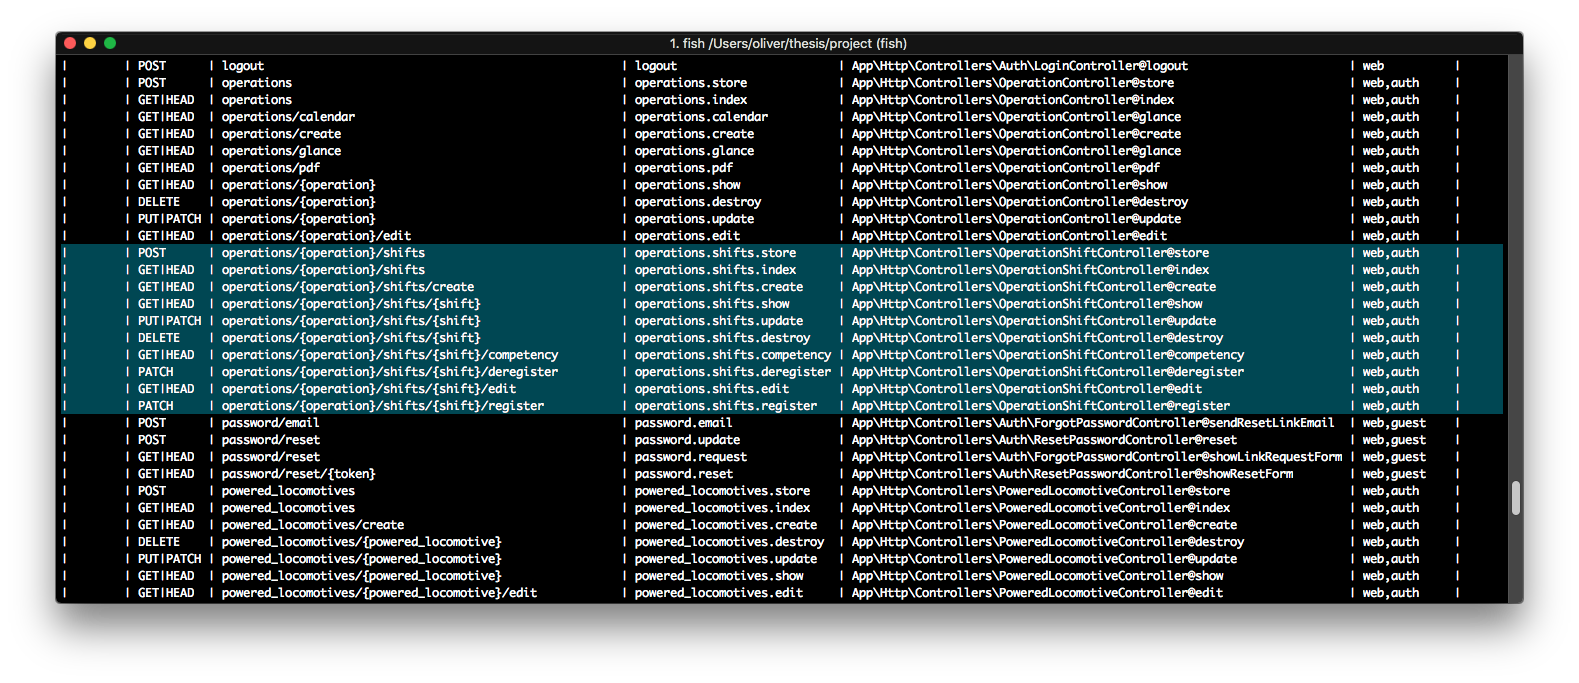
\includegraphics[width=1.0\textwidth]{Figures/nested-components}
    \caption{Screenshot showing how nested components (operations and shifts) appear within Laravel.}
    \label{fig:nested}
\end{figure}

All operations can be viewed in a reverse-chronological, paginated view, or individual operations and their shifts can be viewed independently. This is one of three primary ways of viewing shift availabilities and their information, designed to be a more modern, bespoke solution for navigating data in line with early concept artwork. It is important to note that shifts are a nested resource of operation - shifts cannot be viewed individually as they are instrinsically dependent on their operation. How this is represented in Laravel is shown in figure \ref{fig:nested}

Whilst adminstrators have complete control over operations and shifts and as aforementioned, can manually assign users to shifts, regular users are expected to sign up for shifts that they are capable (in terms of role and role competency) to do. This is referred to internally as 'registering', with pulling out of a shift and leaving it vacant as 'deregistering'.

Whilst deregistration is relatively straightforward and generall risk-free, registering for a shift is complex and carries out substantial amounts of validation checks to ensure that a volunteer is eligible to do so. First, the currently authenticated user is checked for administrative privileges. If they have them, they are able to bypass all further checks, as they are expected to ensure that rules are enforced themselves and not be confined by the rules of the system. 

\begin{lstlisting}[language=PHP, breaklines]
    public function register(Operation $operation, $id)
    {
        ...
            $roleCheck = Role::where([
                ['user_id', '=', Auth::id()],
                ['role_type_id', '=', $operationShift->role_type_id]
            ])->first();
            
            if (is_null($roleCheck)) {
                flash()->error('You do not have the required role type.')->important();
                return redirect()->back();
            } else {
                if (!is_null($operationShift->role_competency_id)) {
                    if ($roleCheck->role_competency->tier < $operationShift->role_competency->tier) {
                        flash()->error('You do not have a sufficient competency / grade tier.')->important();
                        return redirect()->back();
                    }
                }
                if (!is_null($operationShift->user_id) && $operationShift->user_id !== Auth::id()) {
                    flash()->error('This shift is not vacant.')->important();
                    return redirect()->back();
                }
            }
        }
        ...
    }
\end{lstlisting}

Otherwise, the user is first retrieved from the database and checked to see if the user has a role associated with them with the required role type. If they do not, then an error is displayed and the user is redirected back. The next check ensures that, if the shift has a competency requirement specified, that the user meets that requirement by having a tier level that is not less than required, and failure is met with the same fate.

Lastly, the system checks that the shift has not already been filled and the user is erronously attempting to overwrite another volunteer's place in the system. While the interface would normally not allow for this, the check has been put into place to protect against malicious or accidental data submission, such as from an old or manipulated form.

With these checks complete, the remainder of the method continues executing, and data is saved to the database using Eloquent, before redirecting the user to a view and alerting them of their success.

\section{Calendar View}

\begin{figure}[!ht]
    \centering
    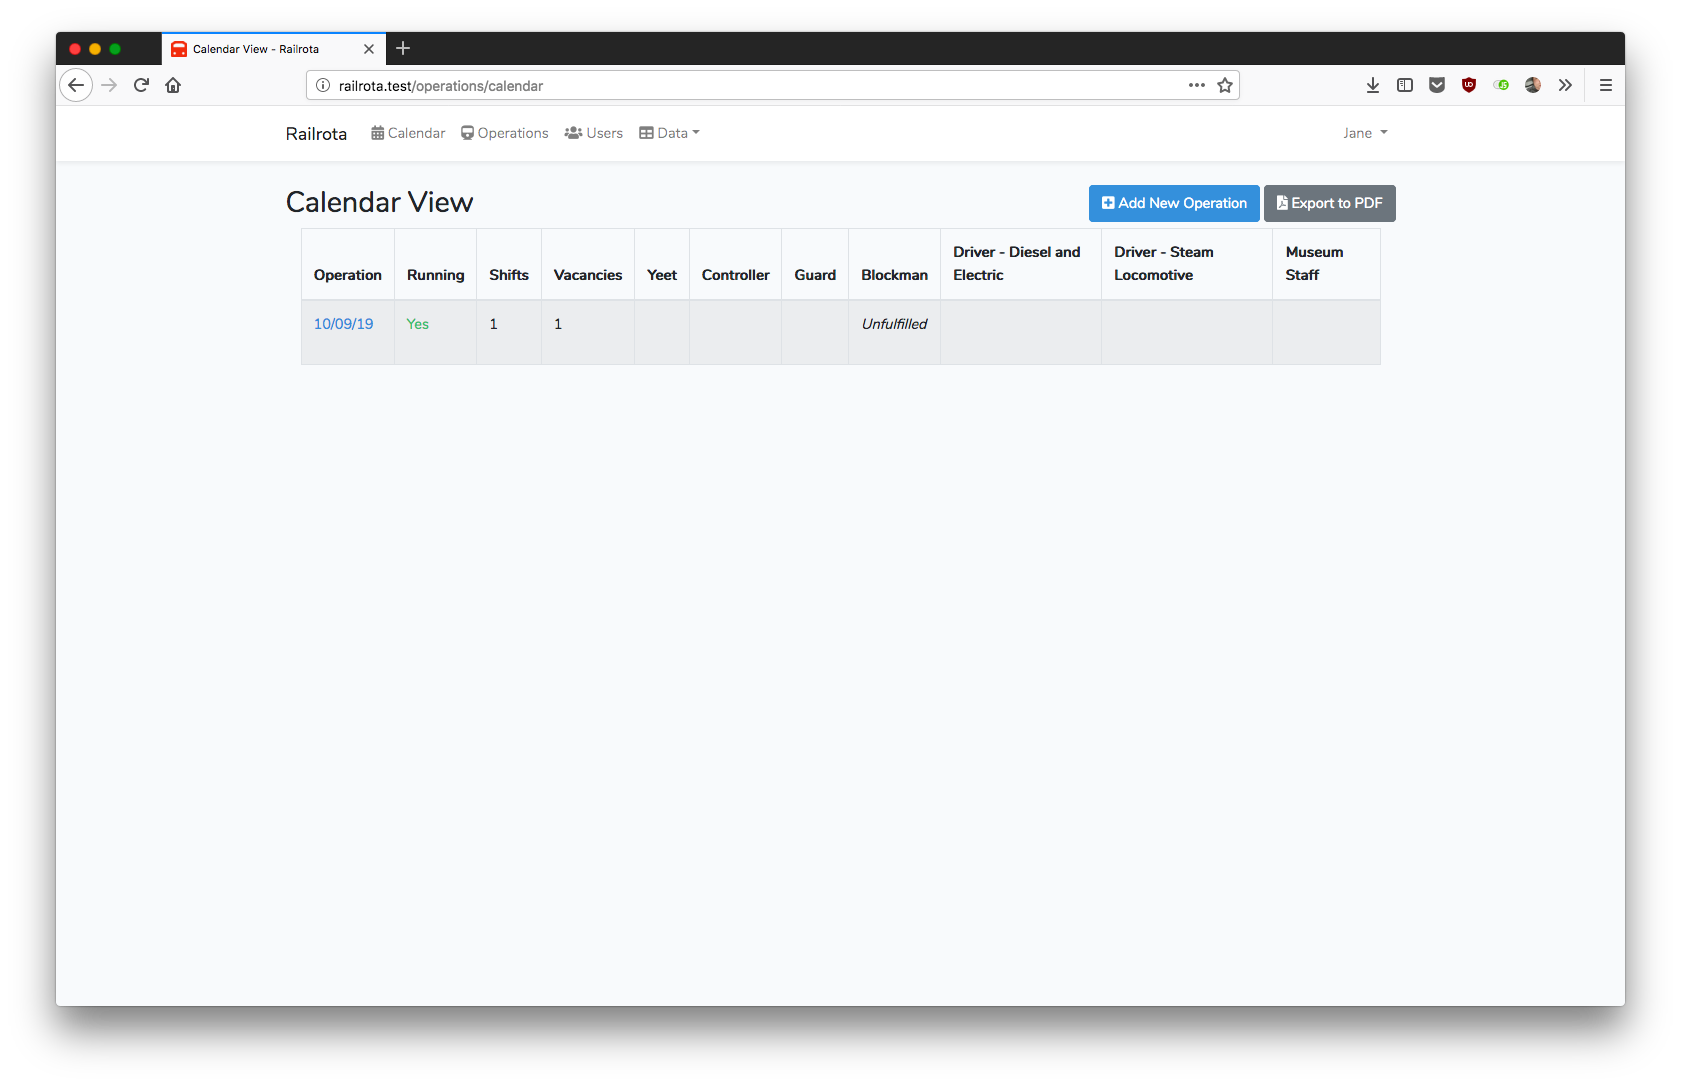
\includegraphics[width=1.0\textwidth]{Figures/screenshot-calendar}
    \caption{Screenshot showing the calendar view, with one operation containing a vacant shift.}
    \label{fig:calendarview}
\end{figure}

Originally coined 'at a glance' view, or just 'glance' view, this functionality was intended to mimic the existing calendar used in Appendix \ref{Example Timetable} to make the transition to the new application easier, and to provide a straightforward means of being able to view vacancies and volunteer staffings en masse. This went through numerous iterations before reaching its current phase, reflected in figure \ref{fig:calendarview}.

Information is spread horizontally, where each operation will contain the names, or a registration link, for vacancies of any shifts running of each type. If there are multiple shifts with the same role type, they will co-exist responsively within the same table field. Historic vacancies - vacancies that went unfilled the day following the operation are labelled as 'unfulfilled'.

\section{PDF Export Functionality}


\section{Administration Panel}

\section{Additional Webpages}